\setchapterimage{Fond_CIN.png}
\setchapterpreamble[u]{\margintoc}

\chapter{Approche énergétique}

\marginnote[4cm]{
\UPSTIcompetence[2]{B2-10}
}

\marginnote[6cm]{\textbf{Emilien Durif}, \textit{Approche énergétique}, Lycée La Martinière Monplaisir, Lyon.}


\section{Introduction}
\subsection{Objectif de la modélisation}
Dans ce chapitre nous aborderons les notions de \textbf{puissance}, \textbf{travail}, et \textbf{énergie}. Ces notions sont fondamentales pour :
\begin{itemize}
\item dimensionner des composants d'une chaîne d'énergie en terme de puissance transmissible;
\item déterminer des équations de mouvement pour prévoir les performances d'un système;
\item estimer le rendement d'une chaîne complète d'énergie.
\end{itemize}



\section{Puissance}
\subsection{Puissance d'une action mécanique extérieure à un ensemble matériel}
\begin{defi}[Puissance d'une action mécanique extérieure à un ensemble matériel]
On définit la \textbf{puissance d'une action mécanique extérieure} à un ensemble matériel $(E)$ en mouvement par rapport à un référentiel $R$ subissant une densité d'effort $\overrightarrow{f}(M)$ (où $M$ est un point courant de $(E)$) comme :

$$
\mathcal{P}(\text{ext} \rightarrow E/R)=\displaystyle{\int_{M\in E}}\overrightarrow{f}(M)\cdot \vectv{M}{E}{R}%(M\in E/R)%\overrightarrow{V}(M\in E/R)
\dd V.
$$
\end{defi}

\begin{remarque}%%[Puissance galiléenne]
On appellera \textbf{puissance galiléenne}, la puissance d'un ensemble matériel $(E)$ en mouvement dans un \textbf{référentiel galiléen} $\rep{g}$ : 
%\begin{align}
%\boxed{
$
\mathcal{P}(\text{ext} \rightarrow E/R_g)
$.
%}
%\end{align}
\end{remarque}%


%\begin{warn}\textbf{Dimensions et homogénéité.}
\begin{marginfigure}[-5cm]
\begin{itemize}
\item Une puissance est une \textbf{grandeur scalaire} s'exprimant en \textit{Watt}.
\item Elle est homogène à un produit entre un effort et une vitesse et peut donc s'exprimer en unité SI en $\text{Nms}^{-1}$.
\item Historiquement on a utilisé longtemps les << chevaux >> ou << cheval vapeur >> ($\SI{1}{ch}= \SI{736}{W}$).
\end{itemize}
\end{marginfigure}

\begin{prop}[Calcul des actions mécaniques s'appliquant sur un ensemble E]
On considère un ensemble matériel $E$ composé de $n$ solides $S_i$. 

Dans la pratique pour calculer la puissance totale des actions mécaniques s'appliquant sur $E$ dans son mouvement par rapport à $R$ il faut sommer toutes les puissances s'appliquant sur les $S_i$ venant de l'extérieur de $E$ :
$$
\mathcal{P}(\text{ext} \rightarrow E/R)=\displaystyle{\sum_{\forall S_i \in E}\mathcal{P}(\text{ext} \rightarrow S_i/R)}.
$$
\end{prop}

%\begin{exemple}[Application sur le système de dépose de composants]
%On considère l'ensemble $E=\left\{S_1+S_2+S_3\right\}$
%
%\question{Construire le graph des liaisons modélisant le système entier.}
%
%\begin{texteCache}
%\begin{center}
%\includegraphics[width=0.9\textwidth]{../../../../sujets/dynamique/depose_composant/images/graph_structure.png}
%\end{center}
%\end{texteCache}
%
%\question{Déterminer l'expression de $\mathcal{P}(\text{ext} \rightarrow E/R_g)$ en fonction de puissances extérieures élémentaires (on ne développera pas les calculs explicitement pour l'instant).}
%\begin{texteCache}
%\begin{align*}
%\mathcal{P}(\text{ext} \rightarrow E/R_g)=\mathcal{P}(S_0 \rightarrow S_1/R_0)+\mathcal{P}(Moteur \rightarrow S_1/R_0)
%+\mathcal{P}(S_0 \rightarrow S_3/R_0)+\mathcal{P}(poids \rightarrow S_3/R_0)
%\end{align*}
%\end{texteCache}
%\end{exemple}

\subsection{Puissance d'une action mécanique extérieure à un solide}
\begin{defi}[Puissance d'une action mécanique extérieure à un solide $(S)$]
La puissance d'une action mécanique extérieure à un solide $(S)$ en mouvement dans un référentiel $R$ peut s'écrire comme le comoment entre le torseur des actions mécaniques que subit $(S)$ et le torseur cinématique du mouvement de $S$ dans le référentiel $R$.

%\begin{align}\label{puissance_action}
%\boxed{
$$
\mathcal{P}(\text{ext} \rightarrow S/R)=\torseurstat{T}{\text{ext}}{S}\otimes \torseurcin{V}{S}{R}.
$$
%}
%\end{align}
\end{defi}



\begin{warn}
On veillera bien, pour effectuer le \textbf{comoment} de deux torseurs, à les avoir exprimé au préalable {\textbf{en un même point.}}
\end{warn}

\begin{remarque}%[Cas particuliers]
\begin{itemize}
\item Le comoment des torseurs est défini par 
$\torseurstat{T}{\text{ext}}{S}\otimes \torseurcin{V}{S}{R}$
$=
\torseurl{\vectf{\text{ext}}{S}}{\vectm{P}{\text{ext}}{S}}{P}
\otimes \torseurl{\vecto{S}{R}}{\vectv{P}{S}{R}}{P}$ 
$=\vectf{\text{ext}}{S}\cdot \vectv{P}{S}{R}+ \vectm{P}{\text{ext}}{S}\cdot\vecto{S}{R}$.

\item Lorsque le torseur cinématique de $S/R$ est un couple (mouvement de translation) alors en tout point $A$ la puissance est alors donnée par
$
\mathcal{P}(\text{ext} \rightarrow S/R)=\vectf{\text{ext}}{S}\cdot \vectv{P}{S}{R} \;
\forall P.
$

\item Lorsque le torseur des actions mécaniques est un torseur couple alors la puissance est donnée par
$
\mathcal{P}(\text{ext} \rightarrow S/R)=\vectm{P}{\text{ext}}{S}\cdot\vecto{S}{R}\;
\forall P.
$

\end{itemize}
\end{remarque}%




\subsection{Puissance d'actions mutuelles entre deux solides}


\begin{defi}[Puissance d'actions mutuelles entre deux solides]
Soient deux solides $(S_1)$ et $(S_2)$ distincts, en mouvement par rapport à un référentiel galiléen $\rep{g}$, et exerçant une action mécanique l'un sur l'autre.
\textbf{La puissance} \textbf{des actions mutuelles} entre $(S_1)$ et $(S_2)$, dans leur mouvement par rapport au repère $R$, est :
$$
\mathcal{P}(S_1 \leftrightarrow S_2/R_g)=\mathcal{P}(S_1 \rightarrow S_2/R_g)+\mathcal{P}(S_2 \rightarrow S_1/R_g).
$$		
 

La \textbf{puissance des actions mutuelles} entre $(S_1)$ et $(S_2)$ \textbf{est indépendante du repère $R$}.
Ainsi,
$$\mathcal{P}(S_1 \leftrightarrow S_2/R)=\mathcal{P}(S_1 \leftrightarrow S_2).
$$
\end{defi}


\begin{remarque}%
\begin{itemize}
\item On peut parler parfois de \textbf{puissance des inter-efforts}.
\item Pour un ensemble $E$, on peut exprimer l'ensemble de la puissance des inter-effort comme la puissance intérieure à l'ensemble $E$ : 
$$
\mathcal{P}_{\text{int}}(E)=\displaystyle{\sum^n_{j=1}}\displaystyle{\sum^{j-1}_{i=1}}\mathcal{P}(S_i \leftrightarrow S_j).
$$
\end{itemize}

\end{remarque}%


\subsection{Puissances d'actions mutuelles dans les liaisons}
\begin{defi}[Puissances d'actions mutuelles dans les liaisons]
Si deux solides $S_1$ et $S_2$ sont en liaison, on a :
$$
\mathcal{P}(S_1 \leftrightarrow S_2) = \torseurstat{T}{S_1}{S_2}\otimes \torseurcin{V}{S_2}{S_1}.
$$

La \textbf{liaison parfaite} si et seulement si quel que soit le mouvement de $S_2$ par rapport à $S_1$ autorisé par la liaison entre ces deux solides, la \textbf{puissance des actions mutuelles entre $S_1$ et $S_2$ est nulle}.
$$
\mathcal{P}(S_1 \leftrightarrow S_2)=0.
$$
\end{defi}


\begin{remarque}%
\begin{itemize}
\item La notion de \textbf{liaison parfaite} s'étend facilement à une liaison équivalente à plusieurs liaisons placées en parallèle et en série entre deux solide $S_1$ et $S_2$. Pour cela il suffit de considérer les torseurs d'action mécanique transmissible et cinématique de la liaison équivalente.
\item L'hypothèse d'une liaison parfaite a pour avantage de mettre en place le théorème de l'énergie cinétique (qui est une conséquence du principe fondamental de la dynamique) sans préjuger de la technologie de la liaison.
\end{itemize}
\end{remarque}%

%
%\section{Travail}
%\subsection{Définition}
%\begin{defi}[Travail]
%Le travail entre deux instants $t_1$ et $t_2$ d'une action mécanique s'exerçant sur un ensemble matériel $E$ dans son mouvement par rapport au repère $R$ est donné par :
%
%$$
%\displaystyle{W^{t_2}_{t_1}}(\text{ext} \rightarrow E/R)=\displaystyle{\int_{t_1}^{t_2}}\mathcal{P}(\text{ext} \rightarrow E/R)\;\dd t.
%$$
%\end{defi}
%
%\begin{remarque}%
%On peut également définir le travail élémentaire par :
%
%$$\dd W(\text{ext} \rightarrow E/R)=\mathcal{P}(\text{ext} \rightarrow E/R)\;\dd t.
%$$
%
%\begin{itemize}
%\item Le travail est une grandeur scalaire.
%\item L'unité de travail est le \textbf{Joule}.
%\item Le travail est homogène au \textbf{produit entre une force et une distance}.
%\end{itemize}
%
%\end{remarque}%
%
%
%
%\subsection{Travail conservatif}
%
%\begin{defi}[Travail conservatif]
%On dit que le \textbf{travail est conservatif} (noté $\displaystyle{{W_c}^{t_2}_{t_1}}(\text{ext} \rightarrow E/R)$) s'il est indépendant du chemin suivi pour passer de l'état initial (instant $t_1$) à l'état final (instant $t_2$).
%Dans ce cas là il existe une grandeur appelée énergie potentielle de l'action mécanique extérieure à $E$ dans son mouvement par rapport à $R$ qui vérifie :
%$\dd W_c(\text{ext} \rightarrow E/R)=-\dd E_p(\text{ext} \rightarrow E/R)$ 
%avec
%$
%\dd W_c(\text{ext} \rightarrow E/R)=\mathcal{P}(\text{ext} \rightarrow E/R)\;\dd t$.
%
%On peut également l'écrire sous la forme :
%$$
%\mathcal{P}(\text{ext} \rightarrow E/R)=-\frac{\dd E_p(\text{ext} \rightarrow E/R)}{\dd t}.
%$$
%\end{defi}
%
%\begin{remarque}%
%\begin{itemize}
%\item On dit que la puissance à travail conservatif dérive d'une énergie potentielle (au signe près).
%\item L'énergie potentielle est une primitive de la puissance. Elle est donc définie à une constante près arbitraire.
%\end{itemize}
%\end{remarque}%
%
%\subsubsection{Énergie potentielle de la pesanteur}
%
%\begin{defi}[Énergie potentielle de la pesanteur]
%L'\textbf{énergie potentielle} associée à l'action de la pesanteur sur un ensemble matériel ($E$) de masse $m$ dans son mouvement par rapport à $R$ est donnée par :
%$$
%E_p(g \rightarrow E/R)=m\;g\;z_G + k.
%$$
%
%Où $z_G$ correspond à la position du centre de gravité $G$ de $S$ suivant la verticale ascendante $\overrightarrow{z}$ (colinéaire au champs de pesanteur $\overrightarrow{g}$) et $k$ une constante.
%
%\end{defi}
%
%
%
%\subsubsection{Énergie potentielle associée à un ressort}
%
%
%\begin{marginfigure}
%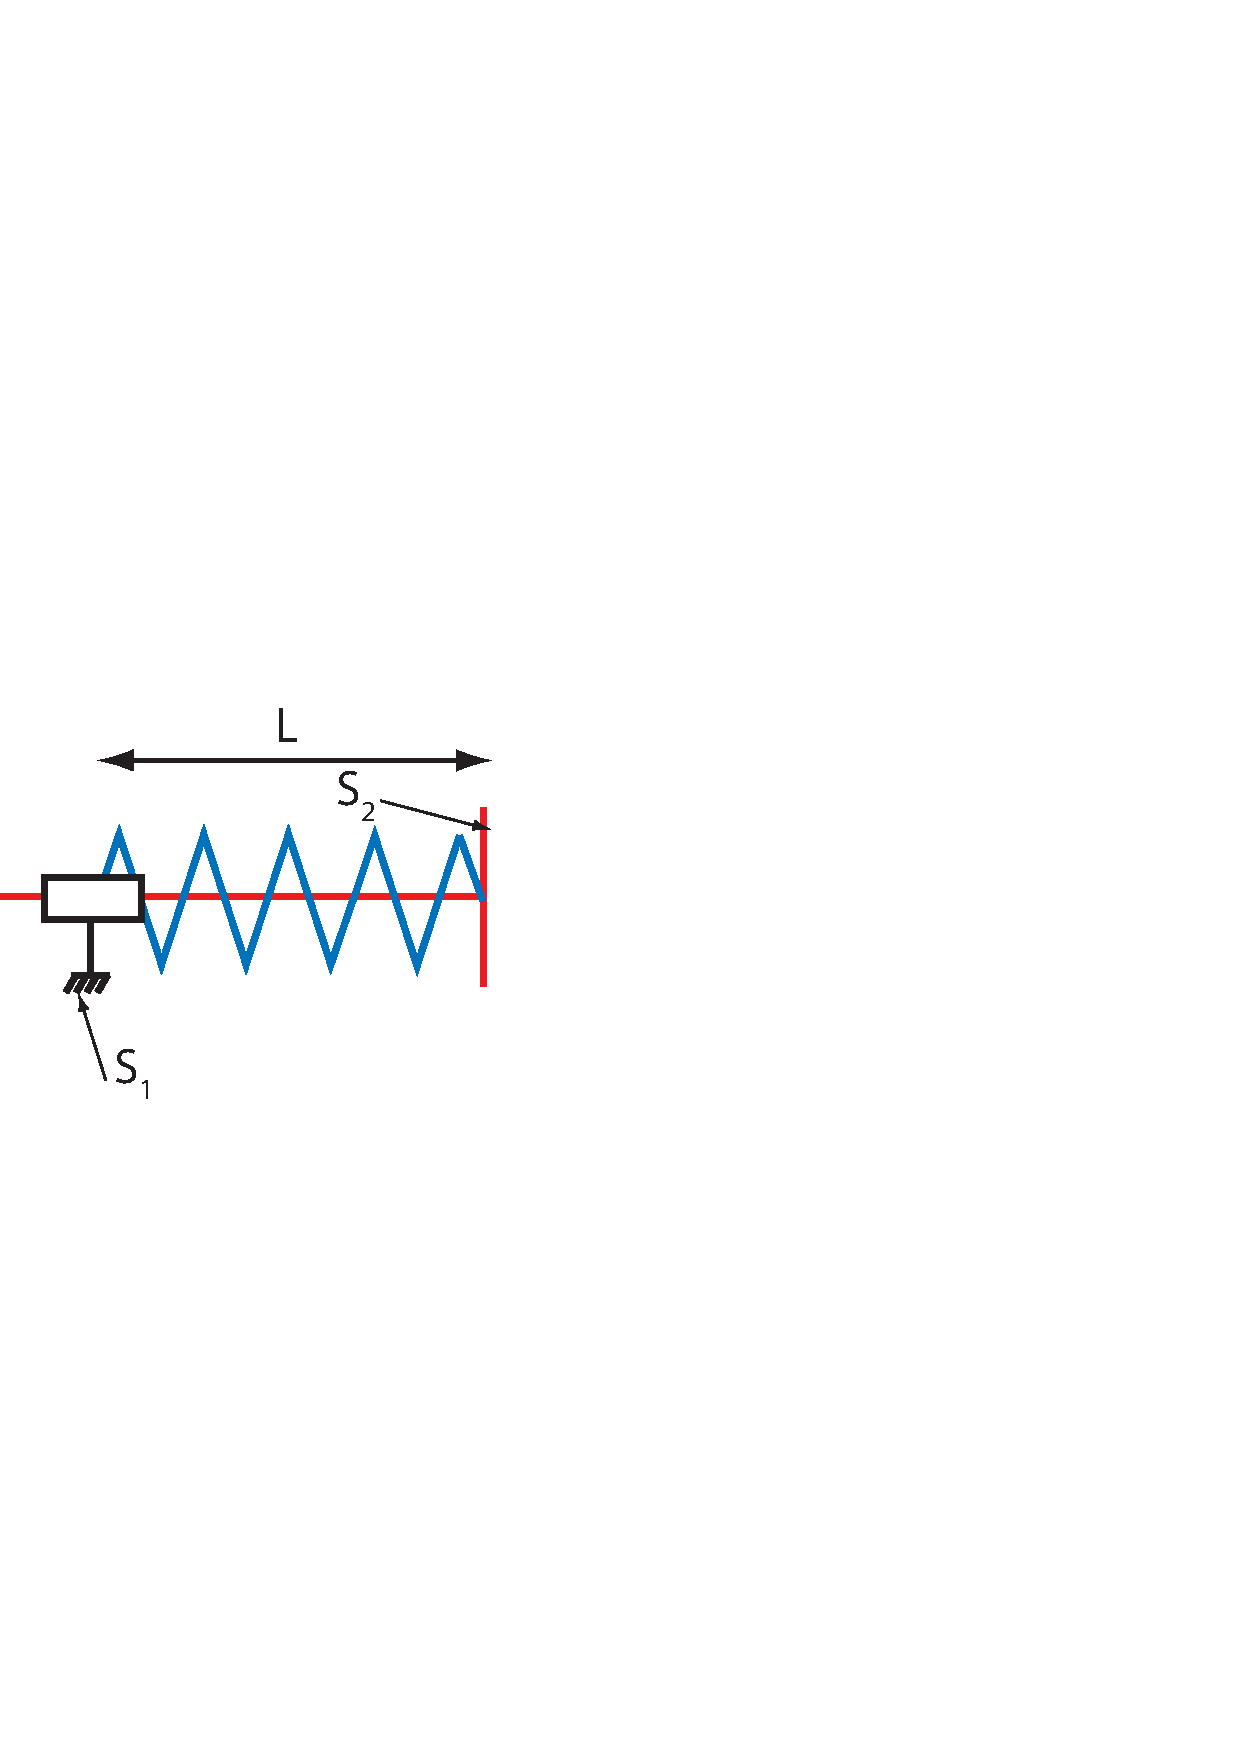
\includegraphics[width=\linewidth]{ressort.pdf}
%\end{marginfigure}
%
%\begin{defi}[Énergie potentielle associée à un ressort]
%
%L'\textbf{énergie potentielle associée à l'action d'un ressort} $r$ de raideur $K$ et de longueur à vide $L_0$ situé entre deux solides $S_1$ et $S_2$ dans son mouvement par rapport à $R$ est donnée par :
%
%$$
%E_p(r \rightarrow S_1,S_2/R)=\frac{K}{2}(L-L_0)^2+k \quad \text{où }k\text{ est une constante}.
%$$
%
%\end{defi}



\section{Énergie cinétique}
\subsection{Définition}
\begin{defi}[Énergie cinétique]
On définit \textbf{l'énergie cinétique} $\ec{S}{\rep{g}}$ d'un système matériel $S$ en mouvement dans un référentiel $\rep{g}$ comme la somme des carrés de la vitesse en chaque point courant $P$ de $S$ pondéré de la masse élémentaire :

$$
\ec{S}{\rep{g}}=\frac{1}{2}\displaystyle{\int_{P\in S}} \left(\overrightarrow{V}(P/\rep{g})\right)^2\;\dd m.
$$

\end{defi}

\subsection{Propriétés}

\begin{prop}[Expression avec les comoments]
L'énergie cinétique peut s'exprimer comme le comoment du torseur cinématique et du torseur cinétique :
$$\ec{S}{\rep{g}}=\frac{1}{2}\torseurcin{V}{S}{\rep{g}}\otimes \torseurci{S}{\rep{g}}.
$$
\end{prop}

\begin{warn}
Il faudra bien veiller à ce que chacun des torseurs soit exprimé en un même point.
\end{warn}

\begin{prop}[Cas particuliers]

\begin{itemize}
\item Solide $S$ de masse $M$ de centre d'inertie $G$ en mouvement de \textbf{translation} par rapport à $R$ :
$$
\ec{S}{\rep{g}}=\frac{1}{2}M \; \vectv{G}{S}{\rep{g}}^2.
$$

\item Solide $S$ de moment d'inertie $I_{Oz}(S)$ en mouvement de rotation par rapport à l'\textbf{axe fixe} $\couple{O}{{z}}$ par rapport $R$ :

$$
\ec{S}{\rep{g}}=\frac{1}{2}I_{Oz}(S)\; \vecto{S}{\rep{g}}^2.
$$

\end{itemize}
\end{prop}



\subsection{Inertie et masse équivalentes}

\begin{defi}[Inertie et masse équivalentes]
Lorsqu'un problème ne comporte qu'un seul degré de liberté et pour simplifier les calculs, on peut exprimer l'énergie cinétique galiléenne d'un ensemble $E$ composé de $n$ solides $S_i$ en fonction d'un seul paramètre cinématique.
On peut alors écrire $\ec{E}{\rep{g}}$ :
\begin{itemize}
\item avec \textbf{son inertie équivalente $J_{\text{eq}}(E)$} (en $\text{kg m}^2$) rapportée à un paramètre de rotation $\dot{\theta}(t)$ : 
$$
\ec{E}{\rep{g}}=\frac{1}{2}J_{\text{eq}}(E) \dot{\theta}^2.
$$
\item avec \textbf{sa masse équivalente $M_{\text{eq}}(E)$} (en $\text{kg}$) rapportée à un paramètre de translation $\dot{x}(t)$ : 
$$
\ec{E}{\rep{g}}=\frac{1}{2}M_{\text{eq}}(E) \dot{x}^2.
$$
\end{itemize}
\end{defi}

\section{Théorème de l'énergie cinétique}
\subsection{Introduction}
Le théorème de l'énergie cinétique est la traduction du Principe Fondamental de la Dynamique d'un point de vue énergétique.
\subsection{Énoncé pour un solide}

\begin{theoreme}[Théorème de l'énergie cinétique]
La dérivée par rapport au temps de l'énergie cinétique d'un solide $S$ dans son mouvement par rapport au référentiel galiléen $\rep{g}$ est égale à la puissance galiléenne des actions mécaniques extérieures à $S$.
Soit :
$$
\dfrac{\dd \ec{S}{\rep{g}}}{\dd t}=\mathcal{P}(\bar S \rightarrow S/\rep{g}).
$$

\end{theoreme}


%\end{document}


\subsection{Énoncé pour un ensemble de solides}

\begin{theoreme}[Théorème de l'énergie cinétique pour un ensemble de solides]
Soit $(E)$ un ensemble de $n$ solide ($S_1$, $S_2$, $\ldots$, $S_n$) en mouvement par rapport à un repère galiléen $\rep{g}$. Le théorème de l'énergie cinétique s'écrit alors :

$$
\frac{\dd \ec{E}{\rep{g}}}{\dd t}=\mathcal{P}(\text{ext}\rightarrow E/\rep{g})+ \displaystyle{\sum^n_{j=1}}\displaystyle{\sum^{j-1}_{i=1}}\mathcal{P}(S_i \leftrightarrow S_j/\rep{g})=\mathcal{P}(\text{ext}\rightarrow E/\rep{g})+\mathcal{P}_{\text{int}}(E).
$$
Avec :
\begin{itemize}
\item $\mathcal{P}_{\text{int}}(E)$ la puissance intérieure à $E$ qui est nulle s'il n'y a pas d'apport d'énergie interne ni de dissipation (liaisons parfaites);
\item $\mathcal{P}(\text{ext}\rightarrow E/\rep{g})$, la puissance galiléenne de $E$ dans son mouvement par rapport à $\rep{g}$.
\end{itemize}

\end{theoreme}

\begin{remarque}%
\begin{itemize}
\item Dans le théorème de l'énergie cinétique, contrairement au principe fondamental de la dynamique, on tient compte de la puissance des actions mutuelles donc internes à l'ensemble matériel $E$ que l'on considère.
\item Ce théorème permet d'obtenir une seule équation scalaire. Cette méthode est donc moins riche que le principe fondamental de la dynamique mais permet d'obtenir quasiment directement les équations de mouvements.
\item Pour obtenir une équation de mouvement (\textit{ie} éliminer les inconnues en actions mécaniques) il faut alors combiner d'autres équations issues des théorèmes généraux de la dynamique.
\end{itemize}
\end{remarque}%


\section{Notion de rendement énergétique}
\subsection{Définition du rendement d'une chaîne fonctionnelle}

Une étude dynamique d'une chaîne fonctionnelle peut se décomposer en deux parties :
\begin{itemize}
\item en \textbf{régime permanent} (variation d'énergie cinétique négligeable): étude des effets dissipatifs pour estimer une puissance nominale des actionneurs;
\item en \textbf{régime transitoire} : évaluation du complément de puissance pour permettre au système de fonctionner.
\end{itemize} 

\begin{defi}[Rendement d'une chaîne fonctionnelle]
Le rendement se définit \textbf{en régime permanent} comme la puissance utile sur la puissance d'entrée d'une chaîne fonctionnelle : 

$$
\eta=\dfrac{\mathcal{P}(\text{utile})}{\mathcal{P}(\text{entrée)}}.
$$

\begin{itemize}
\item $\eta\in\left[0,1\right]$;
\item $\mathcal{P}(\text{entrée})>0$ définit la puissance fournie par l'actionneur \textbf{en régime permanent};
\item $\mathcal{P}(\text{utile})>0$ définit la puissance fournie à l'aval d'une chaîne fonctionnelle (effecteur par exemple) \textbf{en régime permanent}.
\end{itemize}
\end{defi}

\begin{prop}[Rendement global d'une chaîne d'énergie]
Le \textbf{rendement global} d'une chaîne d'énergie comportant $n$ éléments de rendements $\eta_i$ est donné par : 

$$
\displaystyle{\eta=\prod_{i=1}^n\eta_i\leq 1}.
$$

Chacun des rendements successifs $\eta_i$ étant au plus égale à 1, le rendement global est nécessairement inférieur ou égal au plus mauvais rendement.
\end{prop}

\subsection{Détermination d'une puissance dissipée}

\begin{prop}[Estimation des dissipations]
On peut évaluer en régime permanent les pertes ou puissance dissipée à partir de la connaissance du rendement $\eta$ : 
$$\mathcal{P}(\text{dissipée})=(1-\eta)\cdot \mathcal{P}(\text{entrée}).
$$
\end{prop}
